\chapter{Background}
\label{ch:background}

\section{Terminology}
\label{sec:terminology}

A \emph{pictogram} (also called a pictograph) is a simplified figure that resembles and represents a physical object. Pictograms are a common sight in a modern everyday life and are used to warn about dangers, to inform about functionality and to hint about specific characteristics. As such, they can be seen e.g. at traffic signs, danger signs, public toilets and in computers. Naturally, pictograms vary in shapes and sizes, but they are ultimately designed in a way that make them easy to interpret and understand their symbolic meaning.

Given that the application will be used in a hospital setting, the associated terminology will be extended to the application. A \emph{procedure} is a sequence of steps separated from each other. Each \emph{step} contains a background, an avatar and elements related to the procedure in the form of illustrations or pictures, and may feature interactive as well as non-interactive elements.

Story - scene
Comic strip - panel
Procedure - step

\section{Preceding projects}

This project builds upon experience from a bachelor thesis named \emph{PictogramApp} which was based on another project named \emph{Pictogram-me}.

\subsection{Pictogram-me}

Since 2011, associate professor in graphic design Linda Lien and professor in visual communication Ashley Booth have researched on creative usage of pictograms (figures which represent physical objects, see \ref{sec:terminology}). Their artistic research project, named \emph{Pictogram-me}, experiments how pictograms can be used to express complex social messages \parencite{lien2018}. The aim is to illustrate challenging situations that people who have a difficult life may endure. Despite pictograms being flat and simplified, Lien and Booth wanted to show how pictograms also can visualise difficult topics and promote empathy.

Pictogram-me presents a new set of pictograms that are designed for the purpose of the project. In addition, the project has resulted in various concepts including

\begin{itemize}
    \item \emph{PictoBooth}, a photo booth that translates the body and gestures into real life pictograms,
    \item \emph{PictoFont}, a symbol typeface consisting of various pictograms, and
    \item \emph{PictoTheatre}, a small-scale theatre where pictograms can be arranged on a scene. A tablet can be placed behind the scene and function as a background as illustrated in \ref{fig:pictotheatre}.
\end{itemize}

\begin{figure}
    \centering
    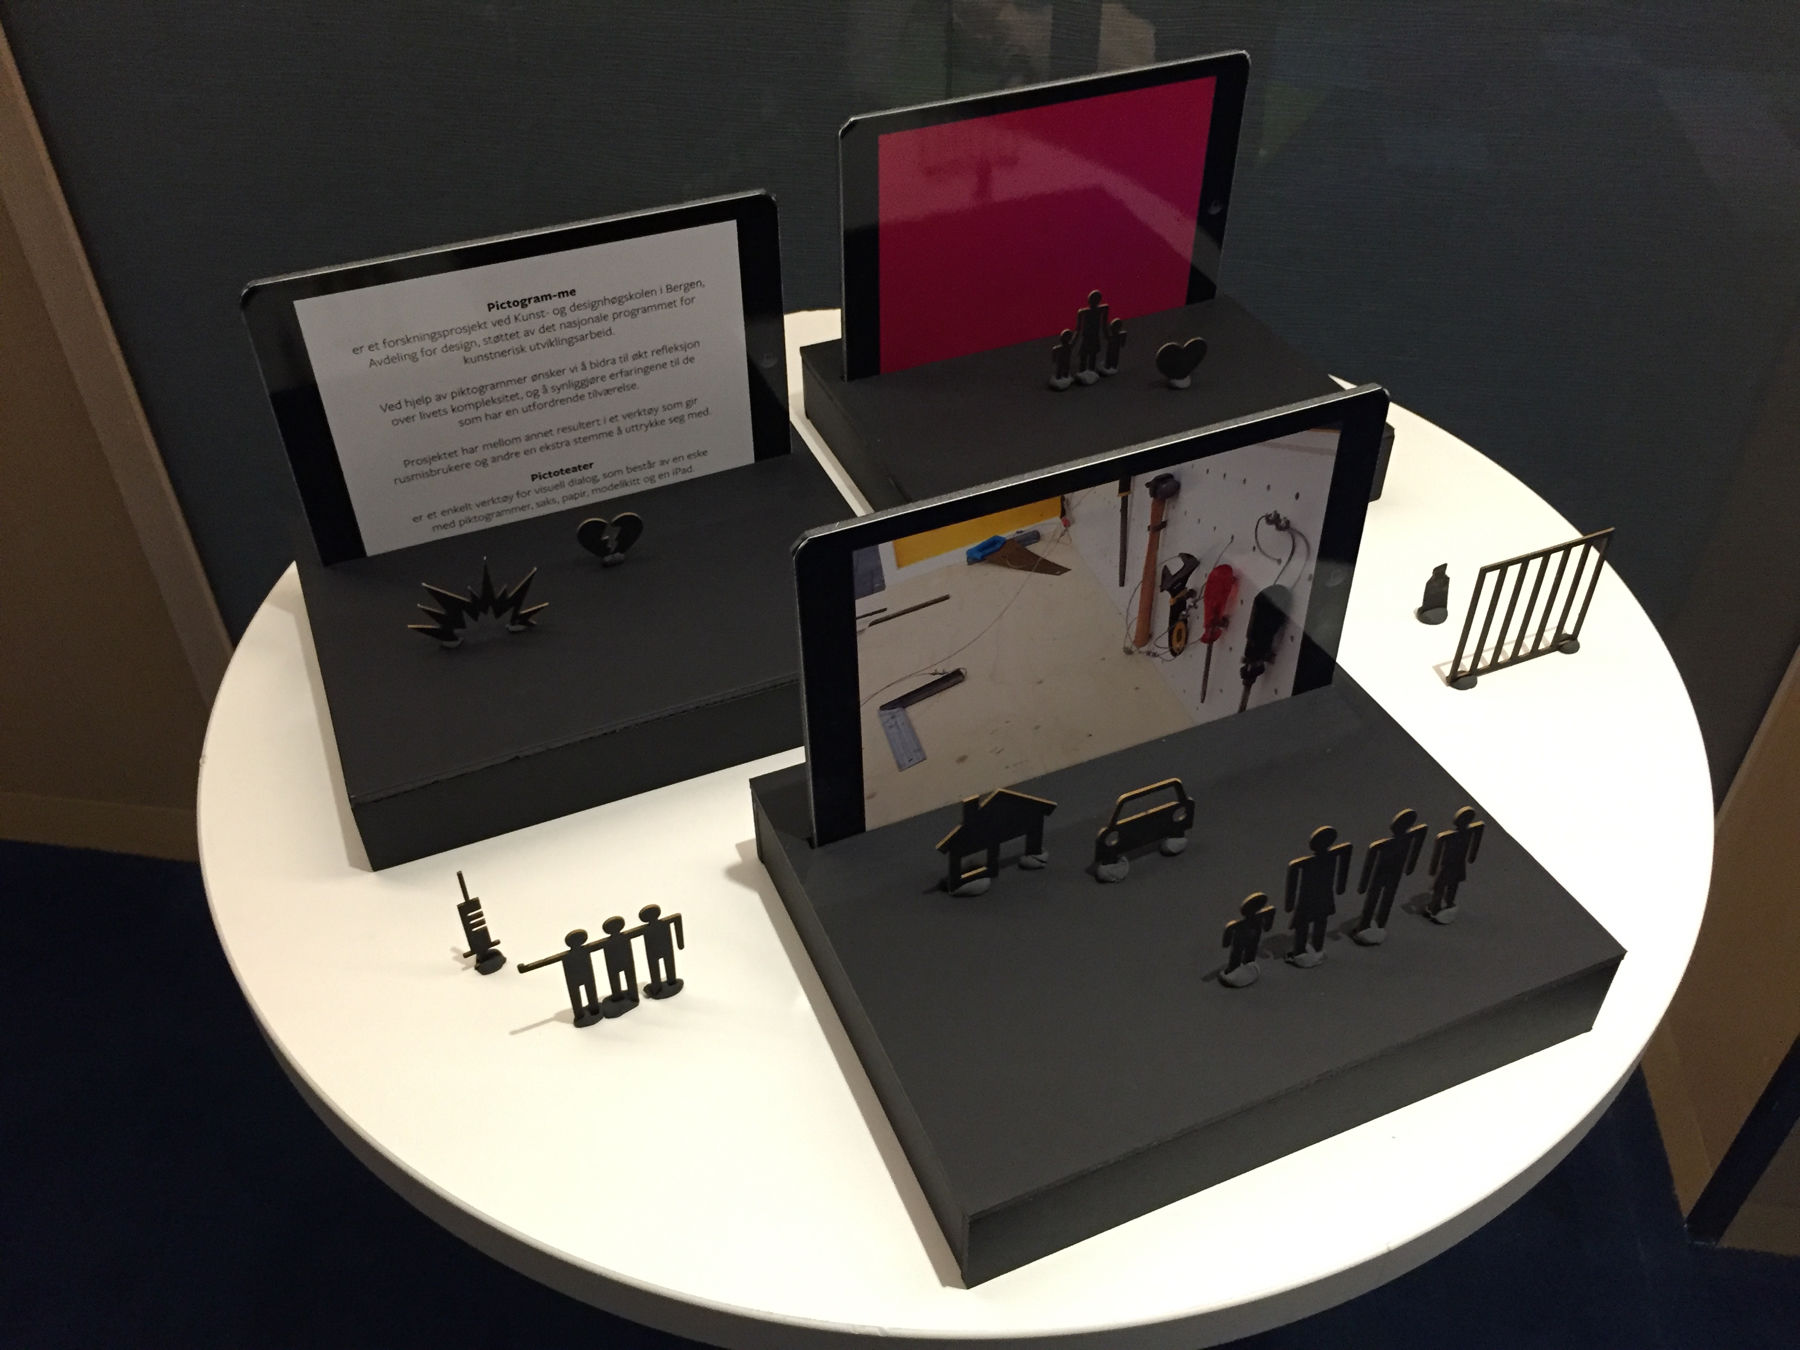
\includegraphics[width=0.55\textwidth]{pictotheatre.jpg}
    \caption{PictoTheatre, shown at the 2016 RØST conference in Bergen}
    \label{fig:pictotheatre}
\end{figure}

\subsection{PictogramApp}

In 2017, the Western Norway University of Applied Sciences issued out a bachelor project in collaboration with Linda and Booth, with the purpose of creating a smartphone application. The application, which was later named \emph{PictogramApp}, was meant to be a digital version of PictoTheatre where pictograms can be arranged on the screen and form visual messages in a mobile manner \parencite{fure2017}. The application allows users to place pictograms in context in order to create their own stories -- see figure \ref{fig:pictogramapp}. PictogramApp was targeted towards the Church City Mission, a voluntary organisation which offers help and services for people living near the street. A functional prototype of the application was released in June 2017.

\begin{figure}
    \centering
    \begin{subfigure}{0.3\textwidth}
        \centering
        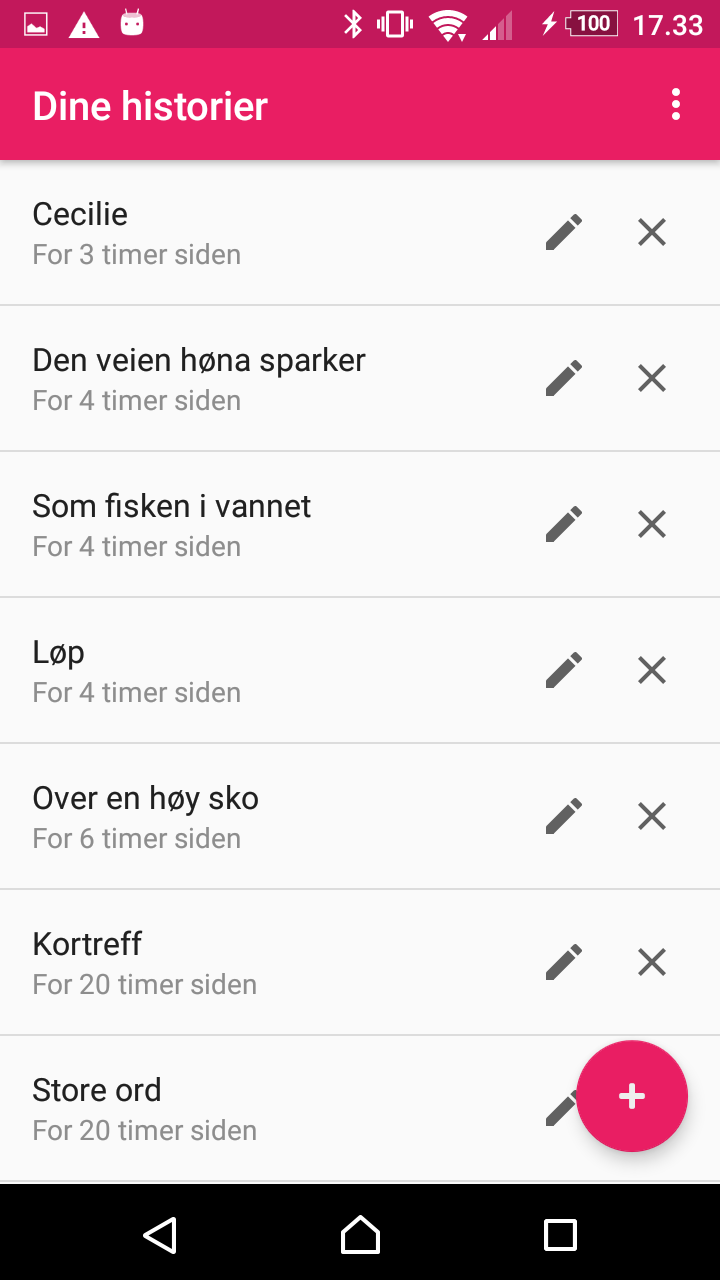
\includegraphics[width=\textwidth]{pictogramapp-01.png}
        \subcaption{List of stories}
        \label{fig:pictogramapp-list}
    \end{subfigure}
    \hspace{0.05\textwidth}
    \begin{subfigure}{0.3\textwidth}
        \centering
        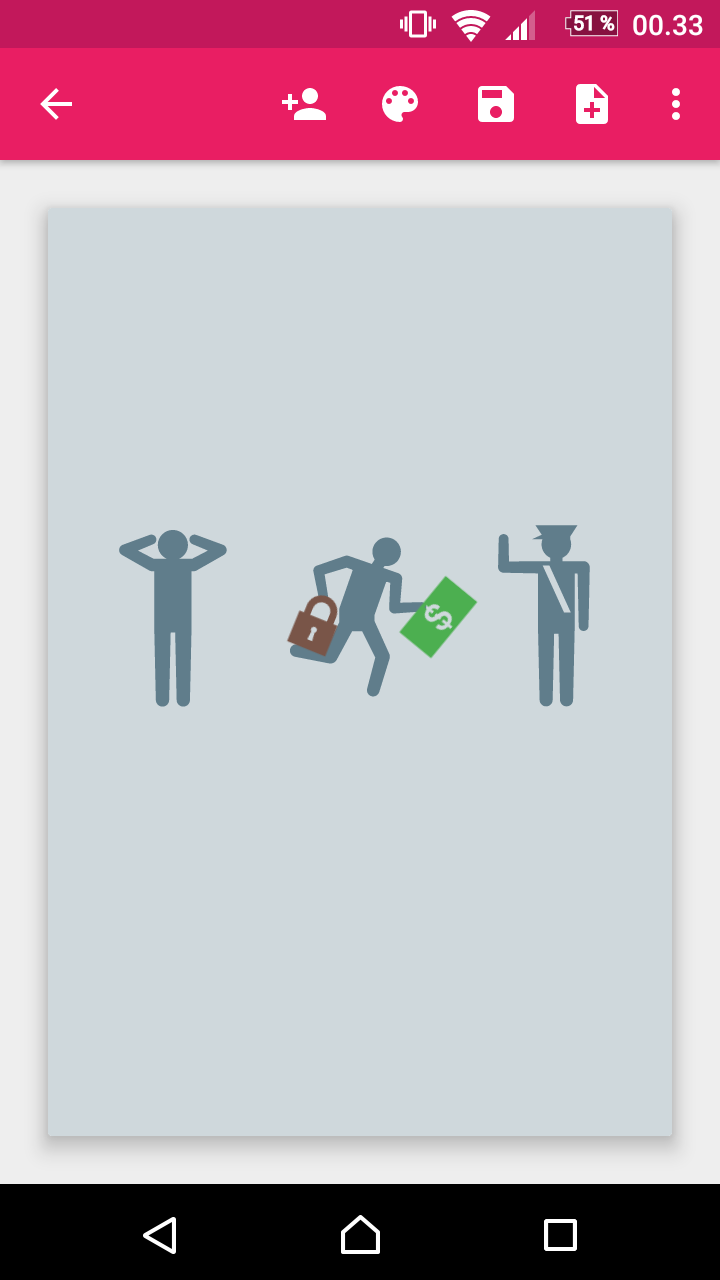
\includegraphics[width=\textwidth]{pictogramapp-02.png}
        \subcaption{Scene editing}
        \label{fig:pictogramapp-scene}
    \end{subfigure}
    \caption{Screenshots from PictogramApp}
    \label{fig:pictogramapp}
\end{figure}

\section{Related work}
\label{sec:relatedwork}

CYC has prior to this project experimented with different ways to engage their patients. Among these was an e-sport event named \emph{E-LAN}, held in the end of October 2018. The purpose of this event was to connect gaming towards a healthy lifestyle and to let children and youth master various areas of interest. As a part of this initiative, an avatar generation system was created that let users create personal avatars which represent themselves. Each user would then carry their avatar in a name tag attached on their clothing. The software seems to run on Windows with support for a web client, and outputs two-dimensional portrait pictures.

Several applications and prototypes have been made that aim to provide information about and illustrate a child's hospital stay. A notable example is \emph{IACTA}, short for \emph{Inter-Active Communication Tool for Activities}. This application ()...) \parencite{stalberg2018}.

Another example is an inpatient portal application named \emph{MyChart Bedside}, developed by Epic Systems Corporation. for tablet devices. A study conducted by \textcite{kelly2017} revealed that 90 percent of children's parents were satisfied with the portal. 

Bitmoji

Instruction videos used by Norwegian on their airplanes

\section{Theoretical foundation}

The problem area was presented first and foremost by CYC. During meetings, Paul Thorsen stated that they wanted to improve the ways of which children were informed about upcoming procedures. Currently, the information that is given here is primarily textual and of varying interest for younger patients.

A number of search queries was performed on academic literature in order to confirm these statements and gain further insight in the problem area. Each query contained a set of the following keywords:

\begin{multicols}{3}
    \raggedcolumns
    \begin{itemize}
        \item Hospital
        \item Patient
        \item Pediatric
        \item Children
        \item Information
        \item Informative
        \item Interactive
        \item Understanding
        \item Comprehension
        \item Engage
        \item Cartoon
        \item Comics
        \item Illustrations
        \item Personalised
    \end{itemize}
\end{multicols}

The queries yielded nine articles which form the theoretical foundation of this thesis.

% List relevant papers that cover the problem area?

\section{Methodology}

This project functions as a pilot study in preparation for a bigger project held at the clinic. It is also a comparative study as it may possibly replace the current way of informing patients. This allows the clinic to run a small-scale project and see how the application compares to the existing system at an early stage with reduced investment and costs.

The development will focus on iterating over designs and prototypes in a user-centered manner. Users, both employees and children at the clinic, will be able to try out the design throughout various phases of its development. This user testing may consist of focus groups and uncontrolled experiments, and the gained experience can be applied in the next development stage. The testing will most likely be restricted to the internal group at first, but a designated test group may be created once the design evolves into prototypes. Elements of Design Thinking might also be considered.

The final prototype will be evaluated by comparing it with the current system. A group of two to six users of the intended age group will be invited to test and evaluate the application while a control group of the same size will test the current system under the same conditions. The users will quantitatively rate the systems by giving scores from one to five in areas such as "fun", "understandable" and "interesting". The project is deemed to be valuable if the users find the application to be more informative and engaging than the current system.

It is yet to be decided if the test groups will consist of children situated at the clinic, i.e. the target group, or children around the same age.
